\chapter{Contexte}
\pagebreak
\section*{Introduction}
Dans ce chapitre nous allons présenter le contexte général dans lequel s’est déroulé le projet de fin d’études décrivant d’une part la société Alten Maroc, son activité, son organigramme et sa fiche technique, d’une autre part le cahier des charges régulant l’accomplissement de ce travail. Ainsi, vers la suite nous allons exposer la méthodologie que nous avons suivi afin d’accomplir ce projet.
\section{Contextedu projet}
\subsection{organisme d'aceuil}
Fondée en 1988, ALTEN est une multinationale Française d’ingénierie et conseil en technologies présente dans 24 pays. En 2017, ALTEN a accompli un turnover de 1,975 Millions d’euros, Elle opère dans plusieurs secteurs dont l’aéronautique, automobile, télécom, énergie et bien d’autres. 
L’industrie automobile est engagée dans une mutation de son rôle et de sa relation avec le consommateur, l’utilisateur final et la société en général. Elle contribue à l’émergence de nouvelles solutions de mobilité individuelle, parfois disruptives. Elle s’impose aussi comme l’interface de nouvelles logiques partenariales. L’innovation et la technologie sont le levier indispensable à ces mutations : les équipementiers automobiles en sont des acteurs-clés, aux côtés de leurs clients constructeurs, mais également de nouveaux acteurs industriels et de services.\\
Pour les années à venir, le secteur automobile concentre ses efforts R\&D sur trois priorités : accélérer le développement de l’électrique, mettre au point les systèmes d’aide à la conduite et la conduite autonome, et enfin déployer les services de mobilité. D’autre part, les industriels profitent de l’essor du e-commerce pour investir le marché de la distribution.
\par
C’est pour cela que plus de 4,200 consultants ALTEN sont mobilisés dans les filiales en France et à l’international sur les projets des plus grands constructeurs et équipementiers européens. Les interventions d’ALTEN tournent autour de trois axes principaux : la capacité à mobiliser ses ressources, à s’engager sur des projets et à adapter rapidement les modes d’interventions, son expertise dans des domaines pointus tels que le contrôle moteur et l’électronique habitacle, et enfin son approche transversale et internationale du secteur.\par

% \begin{itemize}
% 	\item lmsqdkjflqmks
% 	\item fmlkdqsjfmlkq
% \end{itemize}
\begin{figure} [H]
\centering
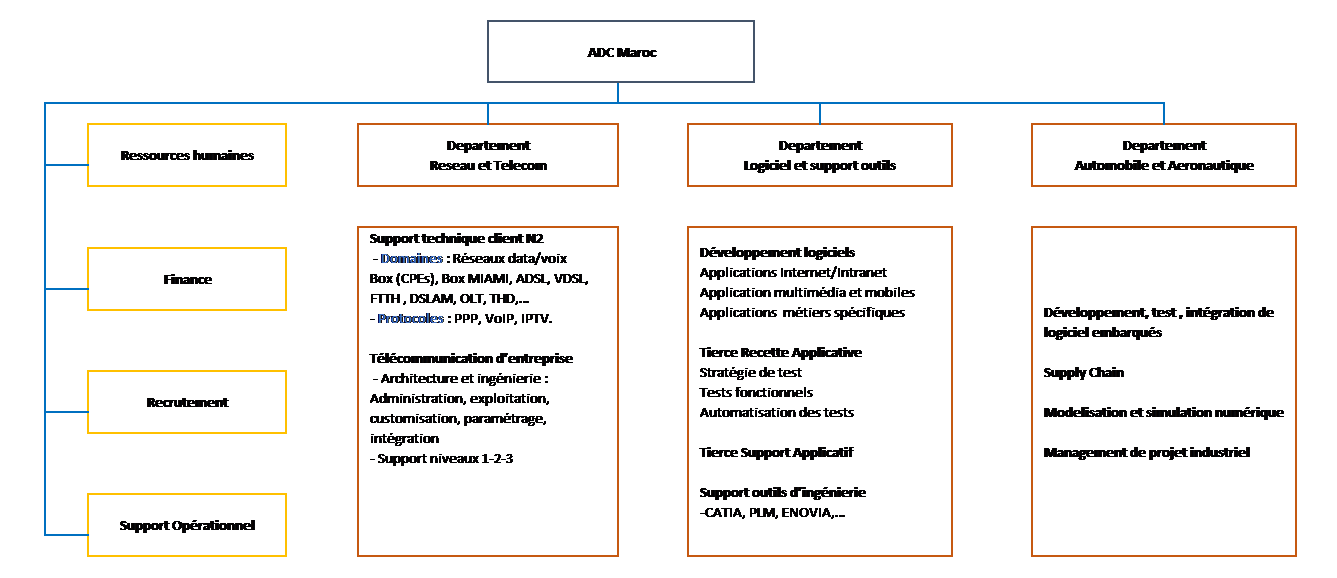
\includegraphics[scale=0.3]{images/organisme}
\caption{figure}
\end{figure}
L’entreprise ALTEN Maroc est divisée en 3 départements :\\
\textbf{Département Logiciel ou Software} : Ce département intervient en conseil ou en réalisation de projets complets dans le domaine de développement logiciel et dans l’assistance applicative.\\
\textbf{Département Réseaux et Télécommunication} : Constitué d’environ 150 consultants, ce service a comme but de gérer le support technique pour les clients de l’opérateur Bouygues Telecom sur toutes sortes de technologies.\\
\textbf{Département Systèmes Embarqués} : constituée d’environ 25 ingénieurs et représente l’équipe où on m’a intégré afin d’accomplir différentes activités et tâches professionnelles. Ce département intervient sur des projets de développement et de test des systèmes embarqués dans le domaine de l’automobile.\\
\begin{figure} [H]
\centering
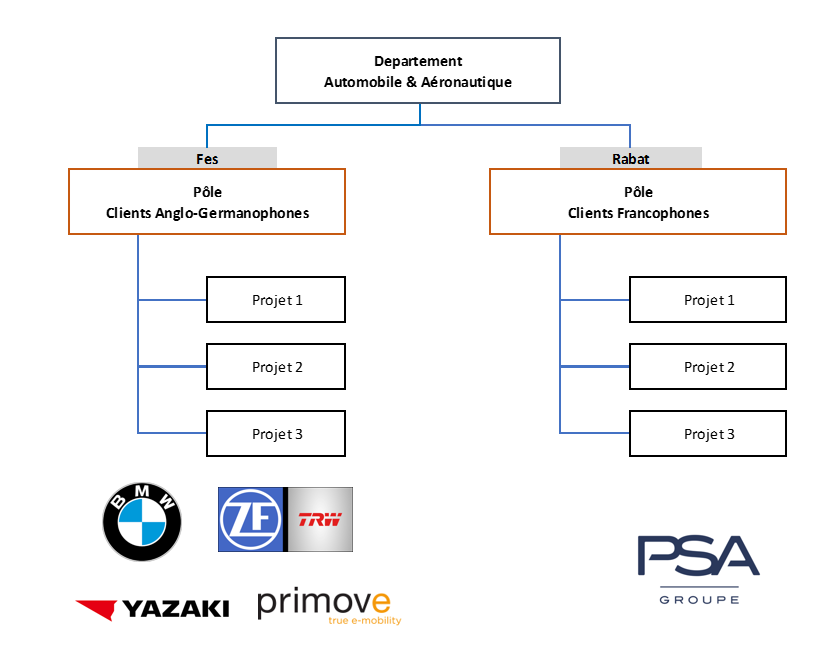
\includegraphics[scale=0.3]{images/departement}
\caption{figure}
\end{figure}
En ce moment, le département Automobile du nouveau site ALTEN Rabat s’occupe principalement des projets Francophones du groupe PSA, alors que celui du Fès travaille sur des projets différents de clients Anglo-Germanophones tels que BMW, Yazaki et Primove.

\subsection{Cadre génerale du projet}
Dans le contexte actuel du marché des logiciels, l’accent est mis sur le coût, le calendrier et les fonctionnalités, la qualité et l’assurance qualité logicielle sont souvent reléguées au second plan. La plupart des développeurs n’appréhendent pas le coût élevé et les retards par rapport aux calendriers inhérents à une mauvaise qualité logicielle. Pour beaucoup d’organismes, la vérification de la qualité n’intervient qu’au moment des essais et une part importante du budget de développement est alors consacrée à corriger les erreurs induites ; souvent, des projets consacrent de 30\% à 50\% de leur budget en coûts de reprise. L’assurance qualité logicielle est un ensemble d'activités planifiées et systématiques, qui soulignent le concept du coût de la qualité mettant en évidence l’importance de la mise en place de méthodes de prévention et d’évaluation afin de réduire les coûts des reprises, de respecter les échéanciers et de satisfaire les demandes du client.\\
Les Hatton, professeur de l’université Kingston de Londres estime qu’en Europe les pertes liées aux erreurs de programmation coûtent jusqu’à 150 milliards d’euros. À travers des tests corrects les dommages pourraient nettement diminuer. Il est plus facile et peu coûteux de résoudre des bugs lors de la programmation du logiciel, par contre lorsque le processus de développement a été effectué, les frais de correction des bugs sont bien plus coûteux. En effet lorsque le logiciel est fini, l’erreur coûte au moins 30 fois plus cher. 


\begin{figure} [H]
	\begin{subfigure}{.5\textwidth}
		\centering
		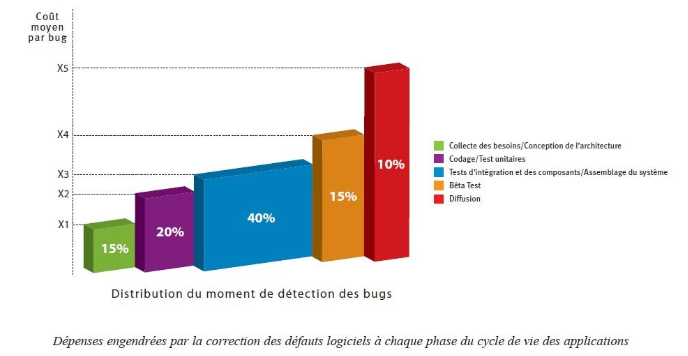
\includegraphics[scale=0.45]{images/cap_1}
		\caption{figure AAAAAAA}
	\end{subfigure}
	\begin{subfigure}{.5\textwidth}
		\centering
		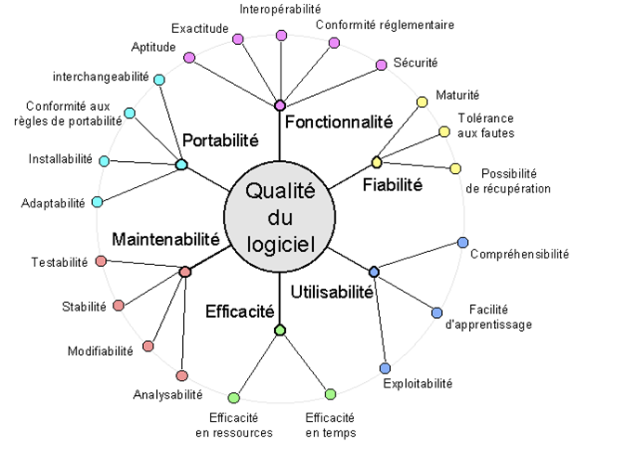
\includegraphics[scale=0.45]{images/cap_2}
		\caption{figure ZZZZZZZZZZZZ}
	\end{subfigure}
	\caption{mlqsdjf}
\end{figure}
Dans le développement de logiciels dans les domaines critiques tels que l’aéronautique, l’automobile, le secteur médical, on essaie de contrôler la qualité à travers des certifications. En effet certaines normes internationales décrivent le processus de développement et le processus de test d’un logiciel. Notamment, Autosar, ISO 26262, CERT et Misra C sont des normes et standards indispensables aussi bien pour les équipementiers, que pour les constructeurs automobiles. Ainsi la qualité du développement de ces logiciels est un enjeu majeur pour garantir le niveau d’intégrité de sécurité, de fiabilité, et de robustesse des systèmes de contrôle-commande. La sûreté de fonctionnement du logiciel évalue que les logiciels, les processus de développement et son environnement d’utilisation respectent les exigences fonctionnelles de sécurité, les normes du domaine et contribuent à la sécurité du système.\\
C’est dans ce contexte globale, que s’inscrit ce projet de fin d’études, avec comme mission la vérification du respect du code de la norme Misra C. En effet Alten vise assurer ces différents clients de la qualité de ces prestations et services pour des projets de test, aussi bien que de développement.
\section{Problematique et objectifs}
Si fabriquer des produits de qualité est une condition nécessaire de compétitivité, ce n’est pas une condition suffisante. L’entreprise d’aujourd’hui se trouve face à l’obligation de fournir un rapport qualité/prix concurrentiel permettant la satisfaction de ses clients et l’augmentation de ses parts de marché. Pour atteindre cet objectif, les industriels se focalisent sur la diminution des charges qui se résume dans le domaine du logiciel par la réduction du nombre de licences payées. Ces licences peuvent avoir un prix élevé et une restriction d’usage très contraignante, donc pour une société multinationale ceci devient une charge importante à réduire.\\
Vector, LDRA , RENSAS, PRQA sont des entreprises mondiaux qui font partie des géant du développement logiciel partie et des principaux fabricants d’outils logiciels pour le test, diagnostic et analyse des systèmes électroniques. Ainsi, ces logiciels sont utilisés énormément dans l’industrie automobile, tel que l’outil QAC, utilisé au sein d’Alten et qui est présent pratiquement chez la plupart des constructeurs et équipementiers en secteur automobile du monde entier.\\
Néanmoins, un inconvénient majeur de cet outil est le prix d’acquisition de sa licence qui avoisine les 170 000 DH par utilisateur, qui reste assez cher et présente une charge pour l’entreprise. Par conséquence la nécessité de trouver une solution alternative afin de remédier à ce problème. Pour ce faire Alten a songé à améliorer l’outil BUSMASTER en y ajoutant les fonctionnalités manquantes tout en augmentant sa robustesse afin de concurrencer l’outil CANoe et de le remplacer par la suite Ce projet entre dans le cadre des projets réalisés au sein de l’équipe de développement software de Lear Corporation Rabat en coopération avec Lear Corporation Valls (Espagne). 
\begin{figure} [H]
\centering
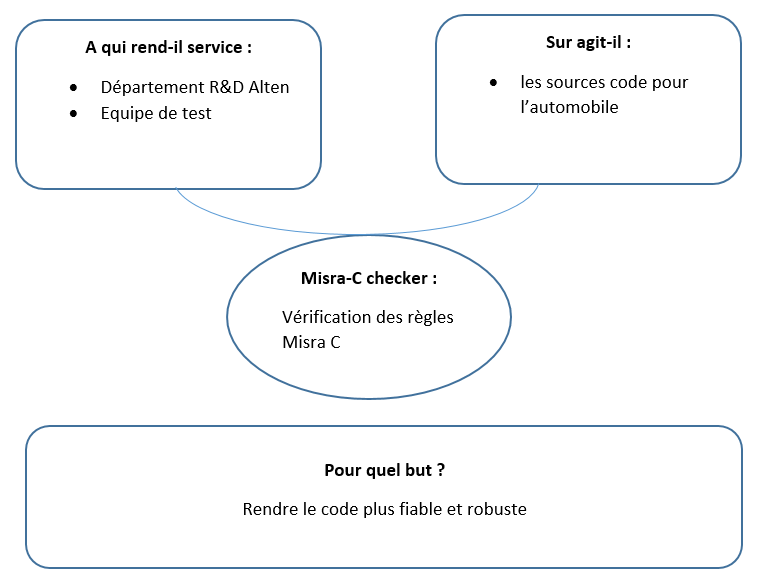
\includegraphics[scale=0.5]{images/cap_7}
\caption{figure}
\end{figure}

\section{Méthodologie et planification}
\subsection{Méthodologie}
Pour garantir le bon déroulement des différentes étapes de réalisation du projet. Il est nécessaire d’adopter une méthodologie de travail qui soit rigoureuse.
Dans notre projet, le modèle a été adopté comme cycle de développement afin d’arriver à termes avec l’approche de mise en œuvre parce que le processus de conception suivant le cycle en V représente désormais la méthodologie standard au sein de la conception de systèmes embarqués.
Son utilisation de la conception au niveau système, d’outils de vérification, et de matériels embarqués standard reconfigurables non seulement permet une réduction du coût et du risque, mais elle aide aussi les équipes à se focaliser sur les nouvelles fonctionnalités en augmentant de façon exponentielle le PPD(les performances par dollar).\\

\begin{figure} [H]
\centering
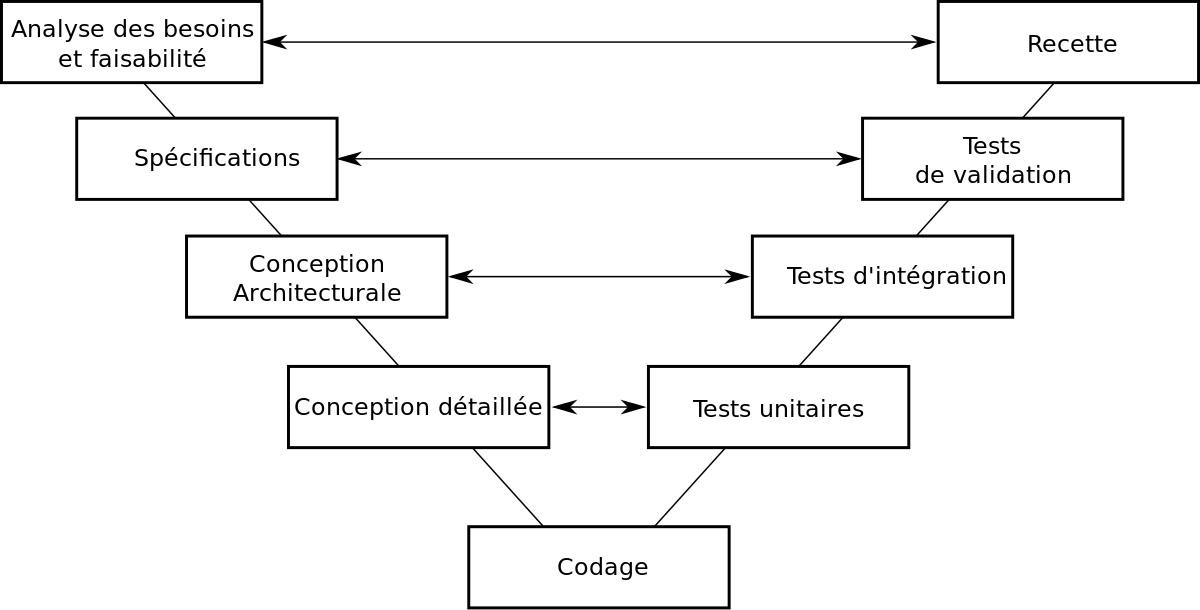
\includegraphics[scale=0.5]{images/cycle}
\caption{figure}
\end{figure}
Le modèle en V demeure actuellement le cycle de vie le plus connu et certainement le plus utilisé. Il s’agit d’un modèle en cascade dans lequel le développement des tests et des logiciels sont effectués de manière synchrone.
Le principe de ce modèle est qu’avec toute décomposition doit être décrite la recomposition et que toute description d’un composant est accompagnée de tests qui permettront de s’assurer qu’il correspond à sa description.\\
Ceci rend explicite la préparation des dernières phases (validation-vérification) par les premières (construction du logiciel), et permet ainsi d’éviter un écueil bien connu de la spécification du logiciel : énoncer une propriété qu’il est impossible de vérifier objectivement après la réalisation.
La représentation en V tient d’avantage compte de la réalité, le processus de développement n’est pas réduit à un enchaînement de tâches séquentielles. Elle montre que :
\begin{itemize}
	\item C’est en phase de spécification que l’on se préoccupe des procédures de qualification
	\item C’est en phase de conception globale que l’on se préoccupe des procédures d’intégration
	\item C’est en phase de conception détaillée que l’on prépare les tests unitaires
\end{itemize}

Le modèle de cycle de vie en V permet d’anticiper sur les phases ultérieures de développement du produit. En particulier le modèle en V permet de commencer plus tôt : Plan de tests de qualification, Plan d’évaluation des performances. Cependant, ce modèle souffre toujours du problème de la vérification trop tardive du bon fonctionnement du système.
\subsection{planification}
La planification du projet fait partie des phases d’avant-projet. Elle consiste à prévoir le déroulement des tâches tout au long des phases constituant le cycle en V qu’on a adopté pour la réalisation de ce projet.
L’utilisation de l’outil de management du projet Gantt permet de schématiser l’enchainement des tâches, ainsi que le chemin critique à suivre pour respecter les délais accordés suivant la planification mise en place.\\
Cette section a pour objectif de détailler les opérations effectuées durant les tâches du planning réel, afin de mieux respecter les délais et les échéances. Ainsi le plan de travail durant ce stage PFE peut être présenté en deux parties principales : l’étude détaillé de l’outils d’analyse statique Cppcheck et l’implémentation des règles du standard Misra C.\\
Le planning du travail réalisé durant le projet est le suivant :


